\documentclass[12pt]{article}
\usepackage[utf8]{inputenc}
\usepackage{amsmath, amssymb}
\usepackage{graphicx}
\usepackage{hyperref}
\usepackage{geometry}
\usepackage{algorithm}
\usepackage{algpseudocode}
\usepackage{amsmath}
\usepackage{mhchem}
\usepackage{booktabs}
\usepackage{subcaption}
\geometry{margin=1in}

\title{Hartree-Fock and MP2 Implementation Report}
\author{Arnav Brahmasandra, Jay Shen, Enoch Woldu}
\date{\today}

\begin{document}

\maketitle

\section{Overview}
The Hartree-Fock method is a foundational approach in quantum chemistry for approximating the electronic structure of atoms and molecules. MP2 provides a post-Hartree-Fock correction to account for electron correlation effects. This report describes the implementation and results of these methods.

\subsection{Code Structure}

\begin{itemize}
  \item \texttt{src/}
  \begin{itemize}
    \item \texttt{molecule.py} – Molecule class representation
    \item \texttt{integrals.py} – Computes 1- and 2-electron integrals using PySCF
    \item \texttt{scf.py} – Restricted Hartree-Fock SCF procedure
    \item \texttt{mp2.py} – Møller-Plesset perturbation theory energy corrections
    \item \texttt{energies.py} – Computing total and nuclear repulsion energies
    \item \texttt{orbital\_plot.py} – 3D visualization of molecular orbitals using PyVista
    \item \texttt{utils.py} – Miscellaneous utilities, including PySCF helper functions
    \item \texttt{plot\_utils.py} – Additional plotting functions.
  \end{itemize}
  \item \texttt{examples/} – Usage demos for common molecules.
  \item \texttt{tests/} – Unit tests and PySCF-based validation.
  \item \texttt{main.py} – A command-line interface to run full SCF/MP2 workflows and visualize selected orbitals.
\end{itemize}

\subsection{Algorithms}

\subsubsection*{Hartree-Fock Self-Consistent Field (SCF)}

The restricted Hartree-Fock (RHF) method approximates the many-electron wavefunction as a single Slater determinant of molecular orbitals. The resulting Hartree-Fock equation can then be solved iteratively by making a mean-field assumption and running a self-consistent field (SCF) procedure. Here, we specifically solve a representation of the Hartree-Fock equation known as the Roothaan equations. 
\[
\mathbf{F} \mathbf{C} = \mathbf{S} \mathbf{C} \boldsymbol{\varepsilon}
\]
We start from an initial guess for the density matrix $\mathbf{P}$, construct the Fock matrix $\mathbf{F}$, and then diagonalize it to obtain molecular orbital coefficients $\mathbf{C}$ and energies $\boldsymbol{\varepsilon}$. $\mathbf{C}$ is used to update $\mathbf{P}$ and the electronic energy can be computed from $\mathbf{P}$ and $\mathbf{F}$. This procedure is repeated until energy convergence. Annotated pseudo-codes for our SCF procedure, as well as the diagonalization of the Roothaan equations, are provided in Algorithms \ref{alg:scf} and \ref{alg:roothaan}. 

\begin{algorithm}
    \caption{Hartree-Fock Self-Consistent Field (SCF) Method}
    \begin{algorithmic}[1]
    
        \Statex \textbf{Input:} Atomic orbital basis set $\{\phi_i\}$; Convergence criteria $\epsilon$
        \Statex \textbf{Output:} Electronic energy $E_{el}$, MO energies $\boldsymbol{\varepsilon}$, MO coefficients $\mathbf{C}$, Density matrix $\mathbf{P}$
        
        \State $G_{ijkl} \gets (\phi_i\phi_j|\phi_k\phi_l)$ \Comment{AO exchange integral matrix from PySCF}
        \State $S_{ij} \gets \langle \phi_i | \phi_j \rangle$ \Comment{AO overlap matrix from PySCF}
        \State $T_{ij} \gets \langle \phi_i \: | \: -\frac{1}{2}\nabla^2 \: |\: \phi_j \rangle$ \Comment{AO kinetic energy matrix from PySCF}
        \State $V_{ij} \gets \langle \phi_i \: | \: -\sum_k^{\text{nuclei}} \frac{Z_k}{r_k} \: | \: \phi_j \rangle$ \Comment{AO nuclear potential energy matrix from PySCF}
        \State $H_{ij} \gets T_{ij} + V_{ij}$ \Comment{Core Hamiltonian matrix}
        \State $P_{ij} \gets 0$ \Comment{Density matrix}
        
        \While{$\Delta E_{el} > \epsilon$}
            \State $F_{ij} \gets H_{ij} + \sum_{kl} P_{kl} \big[ G_{ijkl} - \frac{1}{2} G_{ikjl} \big]$ \Comment{Fock matrix}
            \State $\mathbf{C}, \boldsymbol{\varepsilon} \gets \text{SolveRoothaan} (\mathbf{F}, \mathbf{S})$  \Comment{Compute MO coefficients and energies}
            \State $\mathbf{P} \gets \mathbf{C}\mathbf{C}^T$ \Comment{Update density matrix}
            \State $E_{el} \gets \sum_{ij} P_{ij} (H_{ij} + F_{ij})$ \Comment{Compute electronic energy}
        \EndWhile
        \State \textbf{return} $E_{el}$, $\boldsymbol{\varepsilon}$, $\mathbf{C}$, $\mathbf{P}$
    \end{algorithmic}
    \label{alg:scf}
\end{algorithm}

\begin{algorithm}
    \caption{Solving the Roothaan equation $\mathbf{FC} = \boldsymbol{\varepsilon}\mathbf{SC}$ via diagonalization}
    \begin{algorithmic}[1]
        \Statex \textbf{Input}: Fock matrix $\mathbf{F}$; Overlap matrix $\mathbf{S}$
        \Statex \textbf{Output}: MO coefficient matrix $\mathbf{C}$

        \State $\mathbf{F}' \gets \mathbf{S}^{-\frac{1}{2}} \mathbf{F} \mathbf{S}^{-\frac{1}{2}}$ \Comment{Move Fock matrix to orthonormal basis}
        \State $\boldsymbol{\varepsilon} \gets \text{Eigenvalues}(\mathbf{F}')$ \Comment{Compute MO energies using NumPy}
        \State $\mathbf{C}' \gets \text{Eigenvectors}(\mathbf{F}')$ \Comment{Compute MO coefficients using NumPy}
        \State $\mathbf{C} \gets \mathbf{S}^{-\frac{1}{2}}\mathbf{C}'$ \Comment{Move MO coefficient matrix out of orthonormal basis}
        \State \textbf{return} $\boldsymbol{\varepsilon}$, $\mathbf{C}$
    \end{algorithmic}
    \label{alg:roothaan}
\end{algorithm}

\subsubsection*{MP2 Energy Correction}

The Møller-Plesset perturbation theory of second order (MP2) systematically includes electron correlation effects neglected by RHF. Given the MOs, the perturbative correction is computed by summing over all possible double excitations from occupied to virtual orbitals. This typically lowers the total energy, yielding more accurate results for systems where electron correlation plays a significant role. An annotated pseudo-code of our implementation is provided in Algorithm \ref{alg:mp2}. 

\begin{algorithm}
    \caption{Computation of MP2 Energy Correction}
    \begin{algorithmic}[1]
        \Statex \textbf{Input:} AO basis set $\{\phi_i\}$; MO coefficient matrix $\mathbf{C}$; MO energies $\boldsymbol{\varepsilon}$
        \Statex \textbf{Output:} MP2 energy correction $E_{MP2}$

        \State $G_{ijkl} \gets (\phi_i \phi_j | \phi_k \phi_l)$ \Comment{Compute AO exchange integrals using PySCF}
        \State $\Gamma_{\mu \nu \lambda \sigma} \gets \sum_{ijkl} C_{i \mu} C_{j \nu} C_{k \lambda} C_{l \sigma} \cdot g_{ijkl}$ \Comment{Compute MO exchange integrals}
        \State $E_{MP2} \gets 0$ \Comment{Initialize energy correction}

        \ForAll{occupied MOs $\psi_\mu$, $\psi_\nu$ where $\mu \neq \nu$ }
            \ForAll{unoccupied MOs $\psi_\lambda$, $\psi_\sigma$ where $\lambda \neq \sigma$}
                \State $E_{MP2} \gets E_{MP2} + \frac{(\Gamma_{\mu \nu \lambda \sigma} - \Gamma_{\mu \nu \sigma \lambda})^2}{\varepsilon_\mu + \varepsilon_\nu - \varepsilon_\lambda - \varepsilon_\sigma}$ \Comment{Update energy correction}
            \EndFor
        \EndFor

        \State \textbf{return} $E_{MP2}$
    \end{algorithmic}
    \label{alg:mp2}
\end{algorithm}


\section{Results}

We applied the Hartree-Fock and MP2 implementation to several small molecules using the STO-3G basis set. The table below reports the computed SCF electronic energy, MP2 correlation correction, and the total MP2 energy (including nuclear repulsion) for each system.

\begin{table}[H]
\centering
\caption{Computed Energies for Test Molecules (STO-3G)}
\begin{tabular}{lccc}
\toprule
\textbf{Molecule} & \textbf{SCF Energy (Ha)} & \textbf{MP2 Correction (Ha)} & \textbf{MP2 Total Energy (Ha)} \\
\midrule
\ce{H2}   & $-1.1167$ & $0.0000$ & $-1.1167$ \\
\ce{H2O}  & $-74.9459$ & $-0.003205$ & $-74.9491$ \\
\ce{NH3}  & $-55.4379$ & $-0.01023$ & $-55.4481$ \\
\ce{CH4}  & $-39.7267$ & $-0.006031$ & $-39.7327$ \\
\bottomrule
\end{tabular}
\end{table}

\vspace{1em}

These values agree closely with reference results from PySCF, validating the correctness of both the integral evaluation and the energy computation pipelines.

\subsection*{Molecular Orbital Visualizations}

Representative molecular orbitals were visualized for each molecule using isosurfaces generated with PyVista. The figures below show the HOMO for each molecule overlaid on its atomic geometry.

\begin{figure}[H]
    \centering
    \begin{subfigure}[b]{0.25\textwidth}
        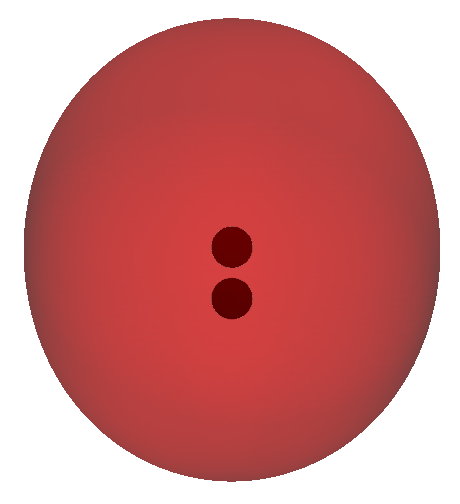
\includegraphics[width=\textwidth]{figures/h2_homo.png}
        \caption{\ce{H2} HOMO}
    \end{subfigure}
    \hspace{1em}
    \begin{subfigure}[b]{0.25\textwidth}
        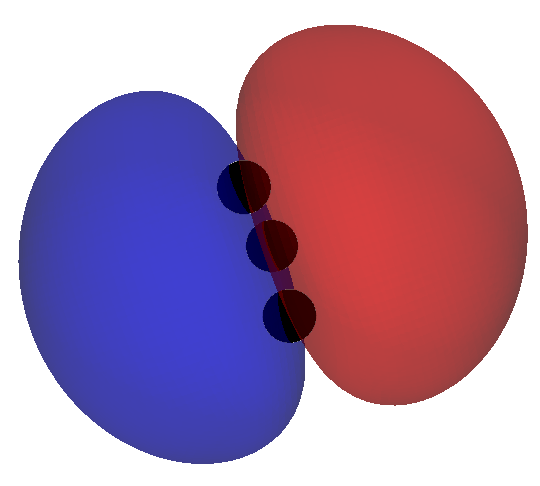
\includegraphics[width=\textwidth]{figures/h2o_homo.png}
        \caption{\ce{H2O} HOMO}
    \end{subfigure}

    \vspace{1em}
    
    \begin{subfigure}[b]{0.25\textwidth}
        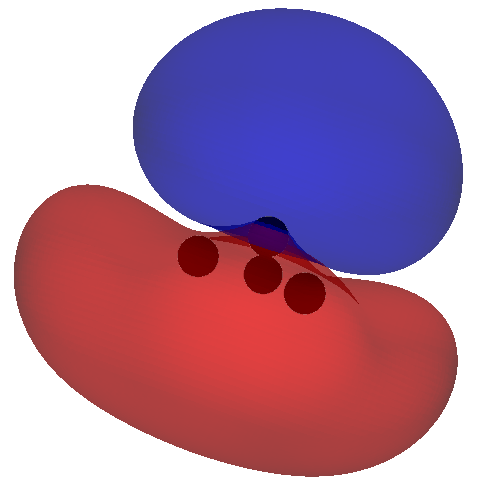
\includegraphics[width=\textwidth]{figures/nh3_homo.png}
        \caption{\ce{NH3} HOMO}
    \end{subfigure}
    \hspace{1em}
    \begin{subfigure}[b]{0.25\textwidth}
        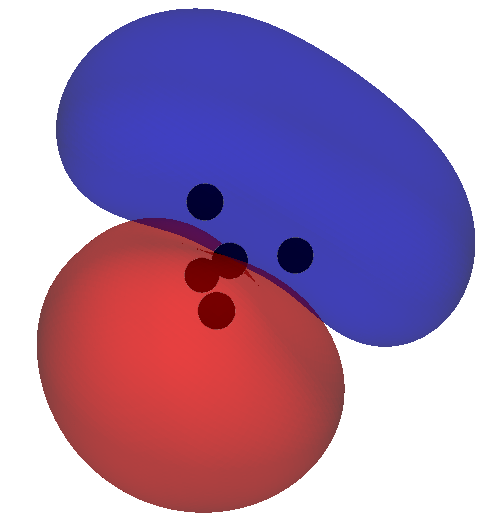
\includegraphics[width=\textwidth]{figures/ch4_homo.png}
        \caption{\ce{CH4} HOMO}
    \end{subfigure}

    \caption{3D visualizations of the HOMOs for each test molecule using isosurface rendering. Blue and red regions represent positive and negative orbital lobes, respectively.}
\end{figure}

\section{Conclusion}

This project presents a compact and functional implementation of Hartree-Fock and MP2 methods from first principles, capable of computing electronic energies and visualizing molecular orbitals for small molecules using the STO-3G basis set. The results show good agreement with reference calculations from PySCF, validating the correctness of the self-consistent field iteration, integral evaluation, and MP2 correlation energy computation.

Despite its correctness and clarity, the current implementation has several limitations. It supports only closed-shell, spin-restricted molecules, relies on a minimal basis set, and uses a memory-intensive four-index transformation for MP2 that limits scalability to larger systems. Future improvements could include open-shell and unrestricted Hartree-Fock support, larger and more flexible basis sets, and density fitting techniques to reduce the cost of MP2. Additionally, implementing more advanced correlation methods such as CCSD(T) or DFT would enhance the accuracy and applicability of the code.

\section*{References}
List references to textbooks, articles, or documentation used.

\end{document}